\documentclass[border=10pt]{standalone}
\usepackage{tkz-euclide}

\begin{document}
    %Based on a figure from O. Reboux with pst-eucl by D Rodriguez.
    %It is not necessary to name the two points that define the mediator.
    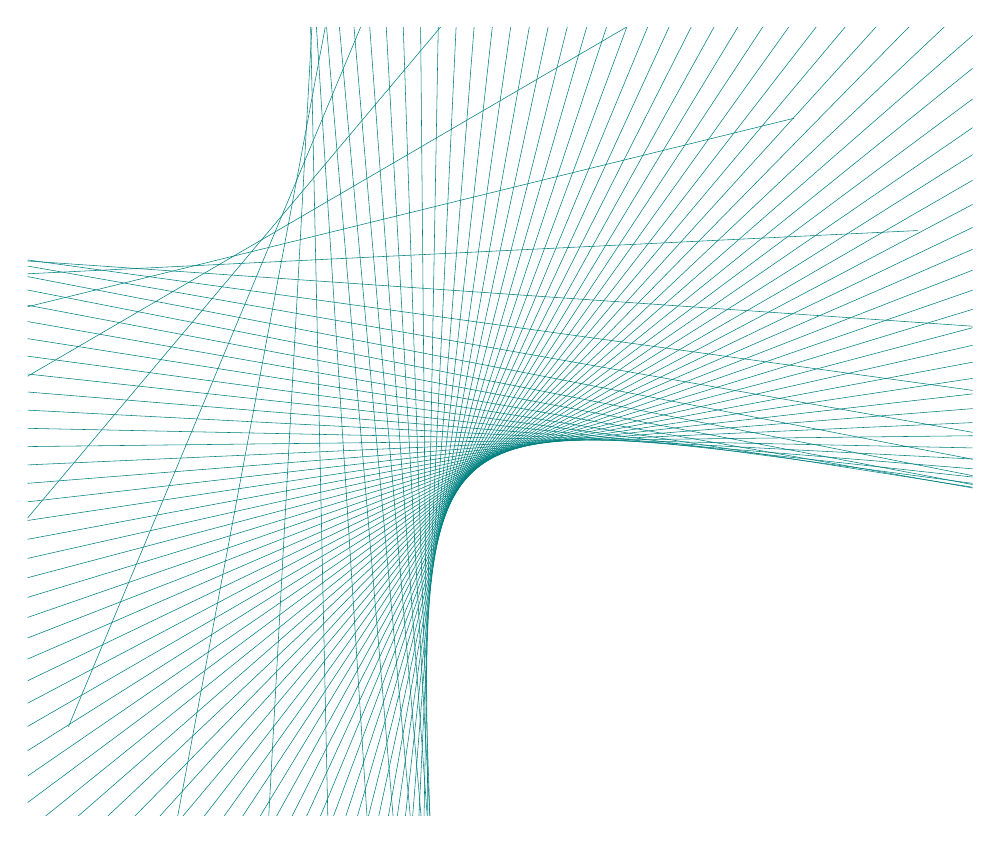
\begin{tikzpicture}[scale=1]
        \tkzInit[xmin=-6,ymin=-4,xmax=6,ymax=6] 
        \tkzClip
        \tkzDefPoint(0,0){O} 
        \tkzDefPoint(132:5){A}
        \tkzDefPoint(4,0){B}
        \foreach \ang in {5,10,...,360}{%
            \tkzDefPoint(\ang:4){M}
            \tkzDefLine[mediator](A,M) 
            \tkzDrawLine[color=teal,add= 3 and 3](tkzFirstPointResult,tkzSecondPointResult)}
    \end{tikzpicture}
\end{document}